この章ではダンピング制御について, その必要性と原理を説明した後, 実際の制御とその効果について記す. 
\section{ダンピング制御とその必要性}
\begin{figure}[H]
\begin{center}
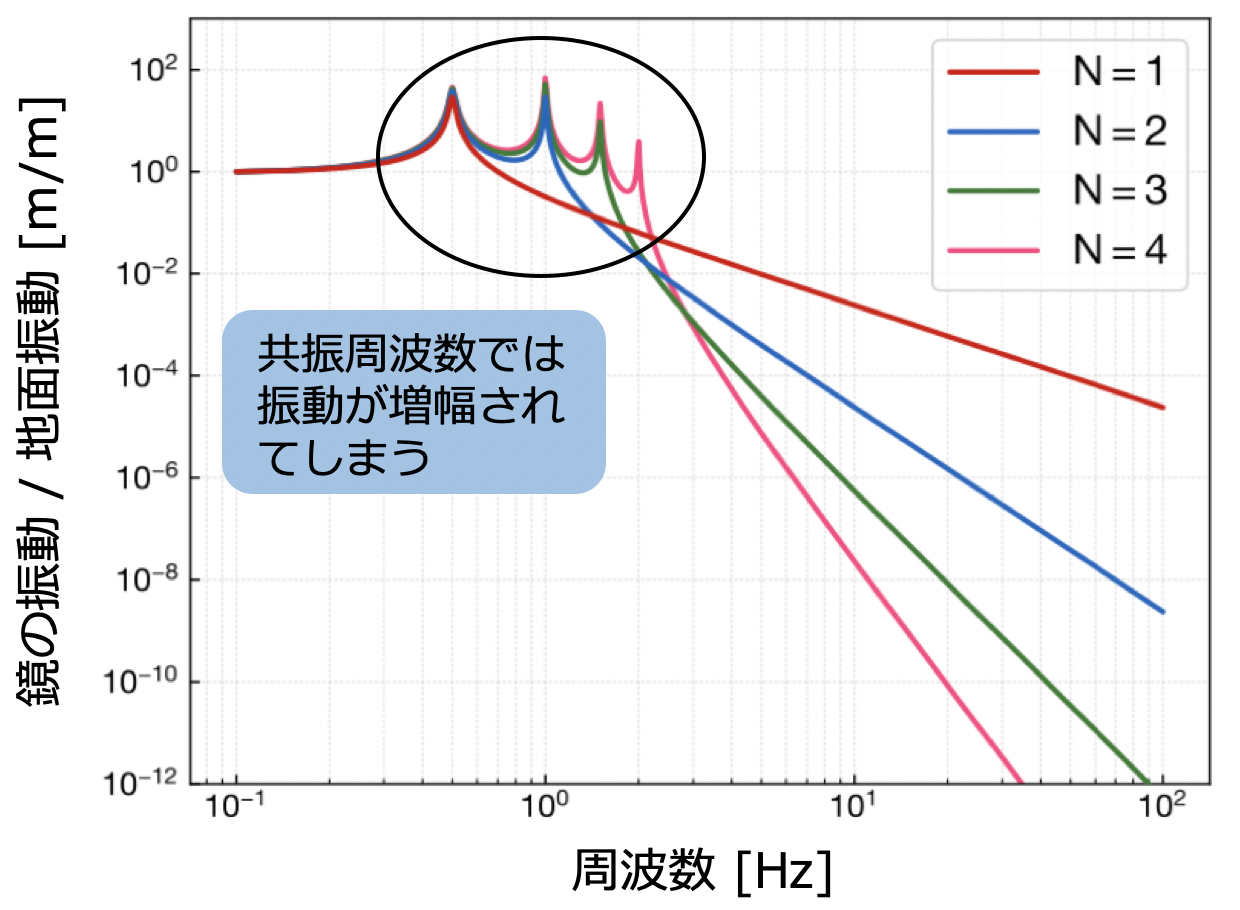
\includegraphics[width=90mm]{fig6_1.png}
\caption[共振周波数における振動の増幅]{多段振り子を用いた防振では共振周波数以上の周波数で高い防振比を得ることができる一方, 共振周波数では鏡に伝わる振動が増幅されてしまう. }
\label{fig6.1}
\end{center}
\end{figure}
第\ref{第3章}章で示した通り, 多段振り子を用いた防振系では共振周波数以上の周波数で高い防振比を得ることができる. その一方で, 共振周波数では鏡に伝わる振動が増幅されてしまう(図\ref{fig6.1}). これでは, 干渉計が安定な状態を保てなくなってしまい, 観測を行うことができない. そこで共振周波数において振動を減衰させるダンピング制御が必要になる. ここで, ダンピング制御とは鏡の変位を局所的にセンサで検出し, それを打ち消す力をアクチュエータによって鏡に加えるフィードバック制御である. つまり, 懸架系にある力(外乱)が加わったとき, 懸架系の応答をフォトセンサが検知し, デジタルシステムに信号を送る. その中でフィルタを通してアクチュエータに信号を送り, 最初に働いた力を打ち消す. そのダイアグラムは図\ref{fig6.2}に示した通りである. 
\begin{figure}[H]
\begin{center}
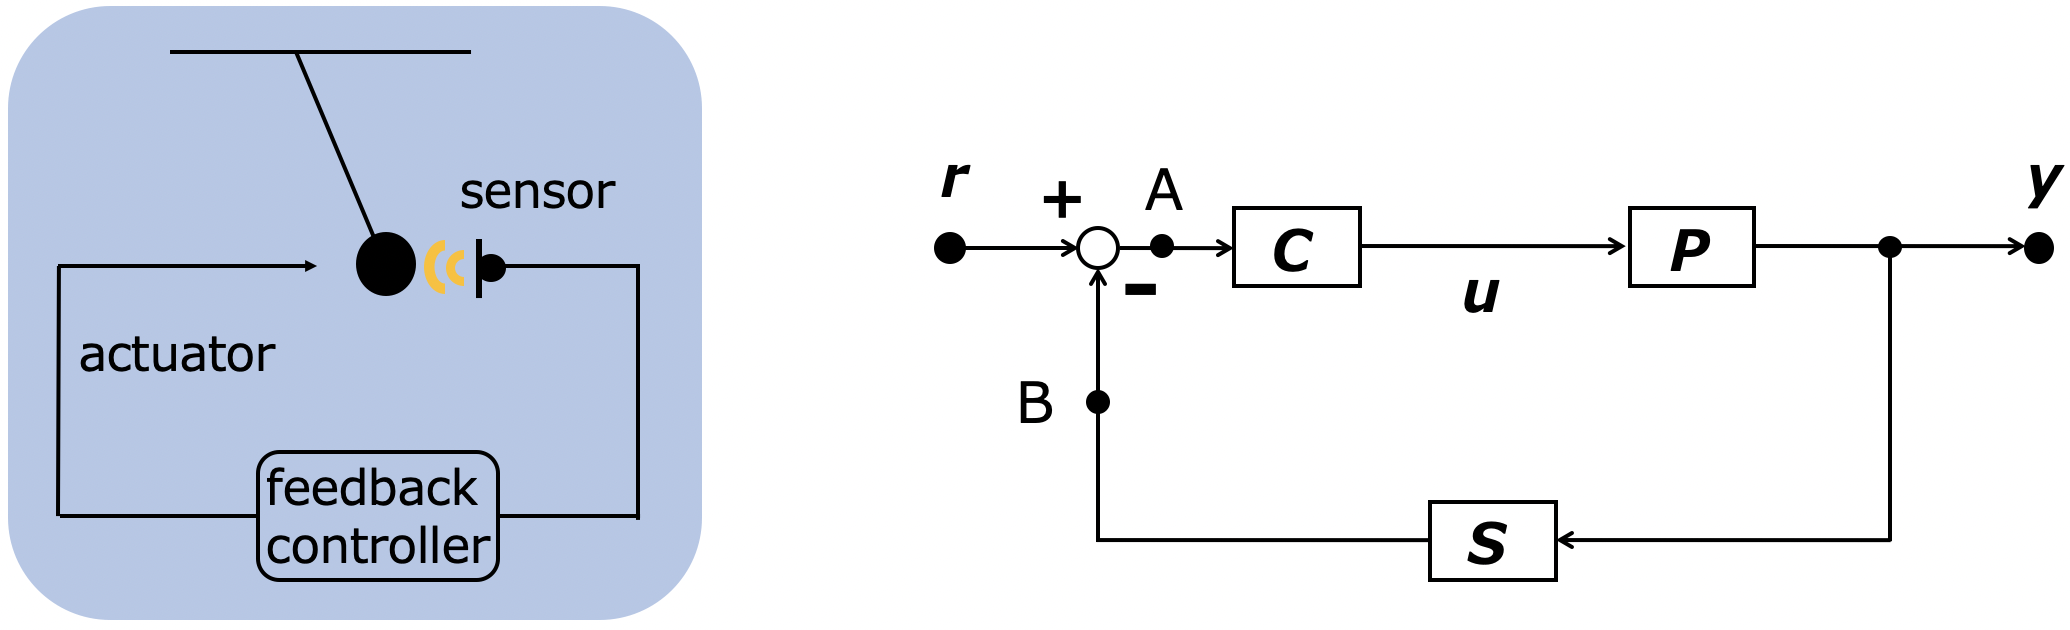
\includegraphics[width=170mm]{fig6_2.png}
\caption[ダンピング制御のダイアグラム]{(左)懸架系のダンピング制御システムの概念図と(右)それと等価なフィードバック制御のブロックダイアグラム. 鏡の変位を局所的にセンサで検出し, それを打ち消す力をアクチュエータによって鏡に加えている. 図中の$C$は制御器, $u$は制御入力, $P$は制御対象, $S$はセンサを表す. また, $r$は目標量, $y$は出力量である.}
\label{fig6.2}
\end{center}
\end{figure}
このときの系の開ループ(open-loop)伝達関数は
\begin{equation}
T_{\rm open}=CP,
\end{equation}
であり, 閉ループ(closed-loop)伝達関数は
\begin{equation}
T_{\rm closed}=\frac{CP}{1+SCP}=\frac{T_{\rm open}}{1+{\rm ST_{\rm open}}},
\end{equation}
と表される. \\
\quad ここで, ダンピングフィルタの実装には一巡伝達関数$ST_{\rm open}$の位相が重要である. ここで, 閉ループではなく開ループ(一巡伝達関数)で考えれば良い理由は以下の通りである. \\
\quad 図\ref{fig6.2}において点Aに単位インパルス\footnote{ディラックのデルタ関数とも呼ばれ, $t\geq0$で連続な任意の関数$f(t)$に対して
\begin{equation}
\int_{-\infty}^{\infty}f(t)\delta(t){\rm d}t=f(0),
\notag
\end{equation}
の作用をする関数である. }を入力したとする. このとき単位インパルスは全ての角周波数成分を含む正弦波のFourier級数に展開できるが, それらの正弦波は点Aから点Bまでの周波数応答特性によって振幅はゲイン倍され, 位相もいくらか遅れて点Bに出力される. \\
\quad このうち位相遅れが$180^{\circ}$である角周波数成分を考える. 位相が$180^{\circ}$ずれているということは正弦波信号の正負が反転するということであるが, 図\ref{fig6.2}において点Bから点Aに戻る際にも正負が反転する. つまり, 点Aに入力された単位インパルスのうち, 位相遅れが$180^{\circ}$である角周波数成分は正負が変わらず点Aに戻ってくる. よってループを一巡したときの振る舞いは扱いの困難な閉ループではなく, 開ループ(一巡伝達関数)を考えれば良い. \\
\quad このとき, $HT_{\rm open}$のゲインが1となる周波数(UGF: Unity Gain Frequency)における位相に気をつける必要がある. \\
\quad 先程と同様に位相遅れが$180^{\circ}$となる角周波数成分を考える. 図\ref{fig6.2}の点Aを出た信号は振幅が開ループのゲイン倍されて戻ってくる. この信号はさらにループを回り, その後も同様に回り続ける. このとき開ループゲインが1より小さければ振幅は減少して閉ループ系は漸近安定になる. 一方で, 開ループゲインが1より大きい場合は振幅が徐々に増大し, 閉ループ系は発散し, 不安定となる. ここで, ナイキスト軌跡(図\ref{fig6.3})が複素数平面上の点(-1+0$j$)を通る場合, 位相遅れが$180^{\circ}$となる角周波数の開ループゲインが1となる. 
\begin{figure}[H]
\begin{center}
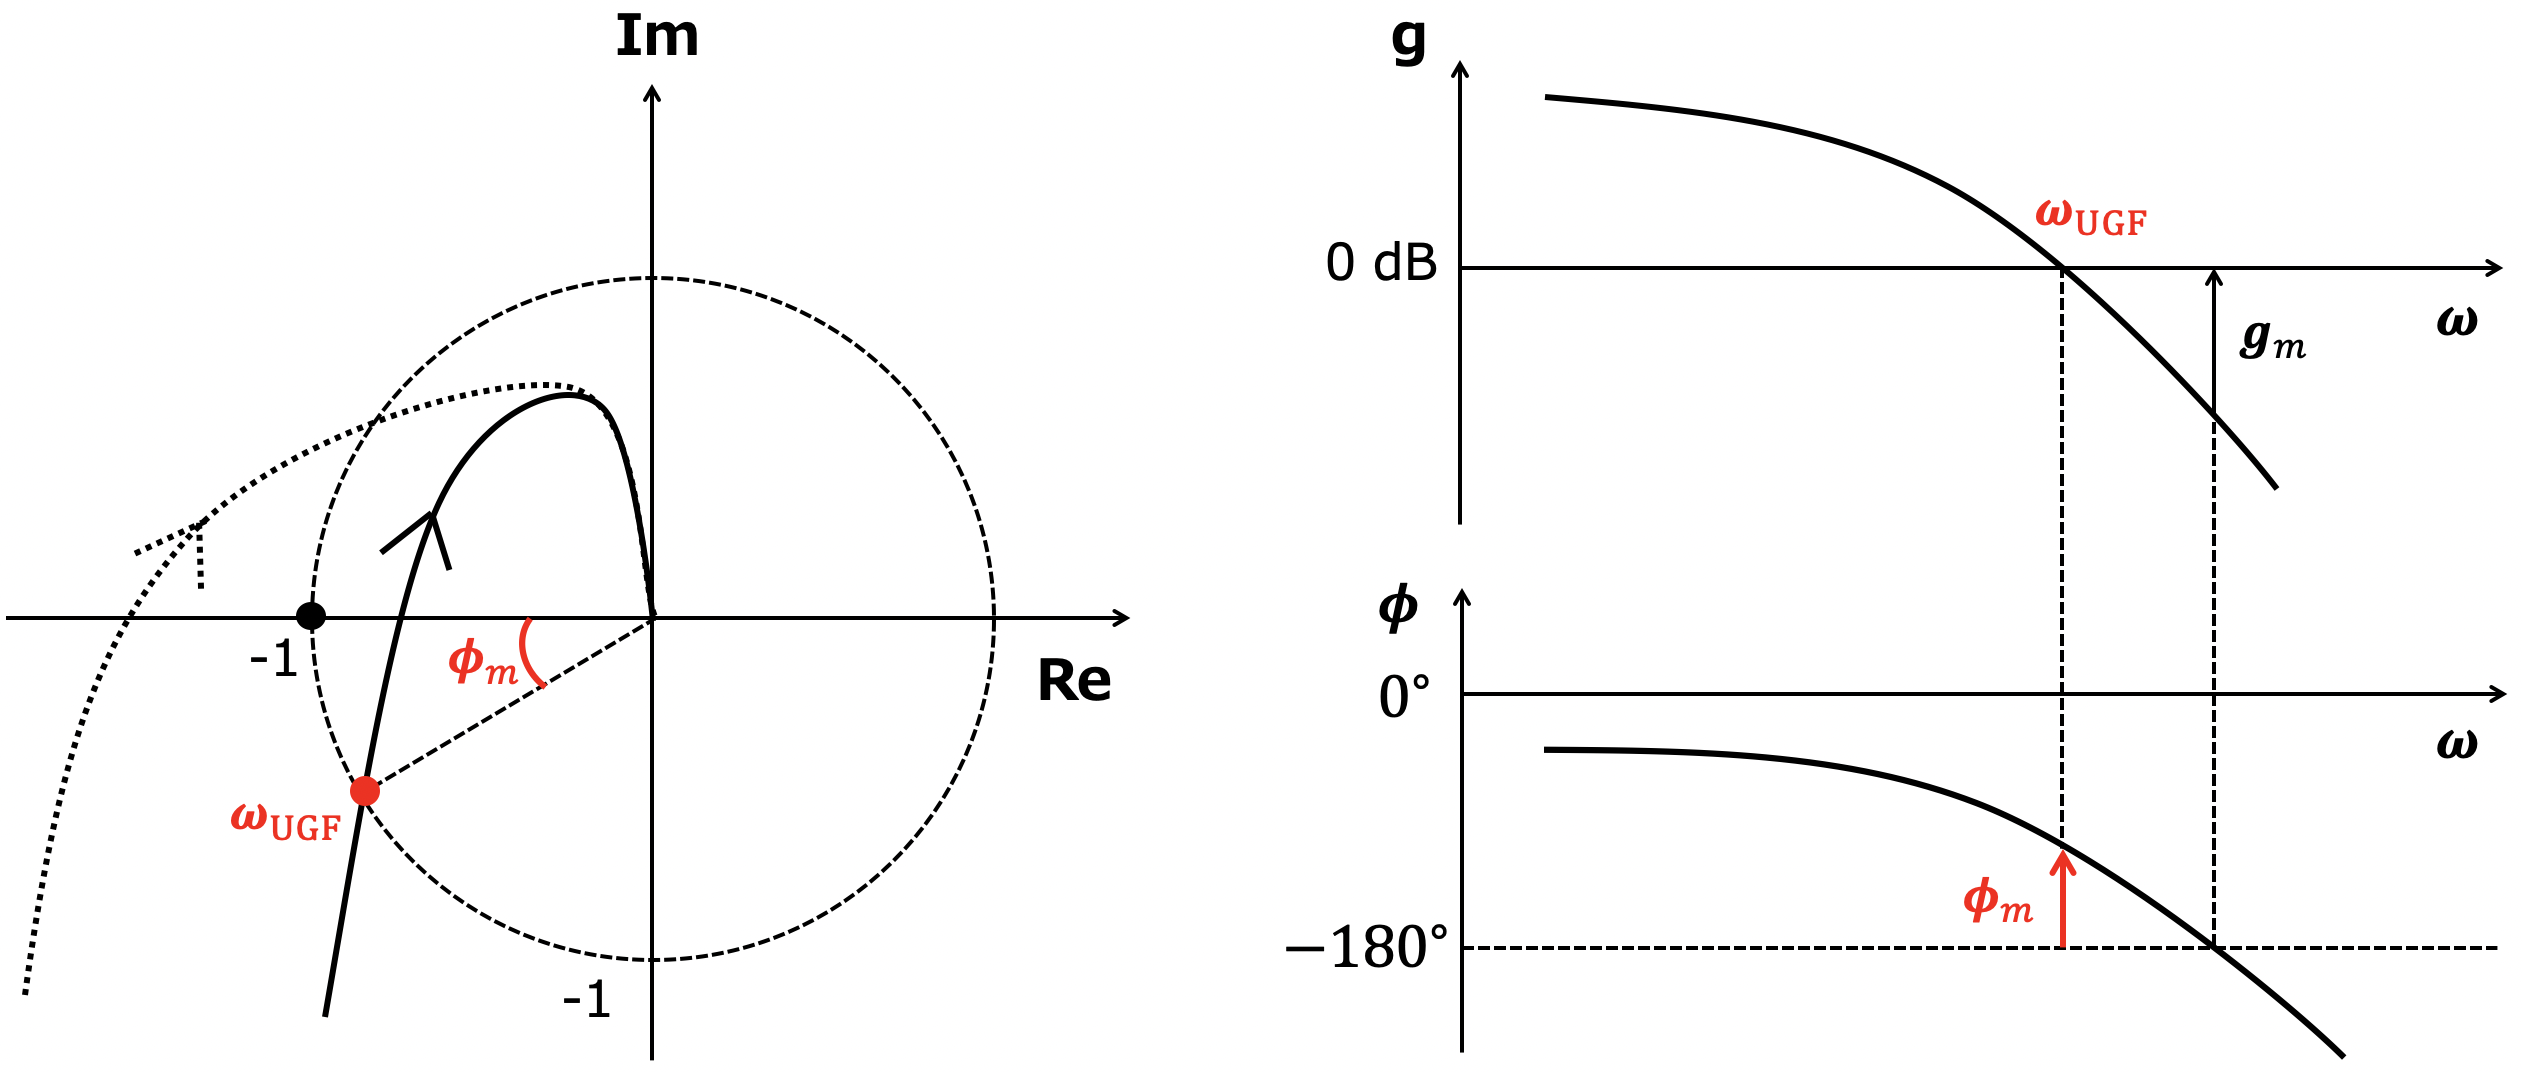
\includegraphics[width=150mm]{fig6_3.png}
\caption[ナイキスト軌跡とボード図]{(左)周波数応答を複素数平面上でベクトルとして表し, その先端を結んで得られる曲線で, ナイキスト軌跡と呼ばれる. UGFはナイキスト軌跡と単位円が交わる点であり, 原点からその点に向かうベクトルの角度を負の実軸から測ったときの角度が位相余裕である. 一巡周波数応答(一巡伝達関数の周波数応答)のベクトル軌跡が(-1+0j)の右側で負の実軸と交われば系は安定, 左側で交われば不安定となる. \\(右)ボード図と呼ばれるもので, 周波数応答と各周波数の関係をゲイン特性曲線, 位相特性曲線で表す. UGFはボード図ではゲイン特性曲線が0 dBの線と交わる点であり, またそのときの位相と-180$^{\circ}$との差が位相余裕である. フィルタを作成する際はボード図を見ながらUGFで位相が180度回っていないか(位相余裕がどの程度あるか)を確認すれば良い. }
\label{fig6.3}
\end{center}
\end{figure}
このときは信号は増大も減少もせず, 点(-1+0$j$)が閉ループ系の安定と不安定の境界となる. つまり, $T_{\rm open}S$のUGFにおいて位相が$180^{\circ}$以上回っていれば, 閉ループ伝達関数$T_{\rm closed}$が発散し, 系のフィードバック制御が成り立たない. \\
\quad すなわち, 安定した系を実現するためには$T_{\rm open}S$のピークにのみゲインを持たせて, このときUGFでの位相が$180^{\circ}$以上回らないようなフィルタを設計する必要がある. ここで, $T_{\rm open}S$に1より大きなゲインを持たせるということは, $T_{\rm closed}$のゲインを下げるということであり, これをダンピングしたい共振周波数に対してのみ行えばよいということである. 
\section{ダンピング制御の原理}
\label{sec6.2}
どのようなフィルタを設計すればよいかをより具体的に考えるために, ダンピング制御の原理について説明する. 先に記述したように懸架系は多段振子であるが, ここでは簡単のため単振子で考える. 速度に比例した項を含めて図\ref{fig6.4}のようなバネで吊るされたモデルを考えと, この系の運動方程式は
\begin{equation}
m\ddot{x}+c\dot{x}+kx=0,
\label{eq6.3}
\end{equation}
となる. ここで$c\dot{x}$は速度に比例した抵抗力である($c$:定数). これを解けば減衰振動に対する解が得られるが, 今は周期的な外力(地面振動など)が加わる強制的な振動を考えるべきであり, この場合式(\ref{eq6.3})は複素数 $z$を用いて
\begin{equation}
\ddot{z}+2\gamma\dot{z}+\omega_0^2z=\omega_0^2a_0{\rm e}^{i\omega t},
\end{equation}
ここで$\gamma=c/2m,\omega_0=\sqrt{k/m}$であり, $a_0:$外力の振幅, $\omega:$外力の角振動数である. 
\begin{figure}[H]
\begin{center}
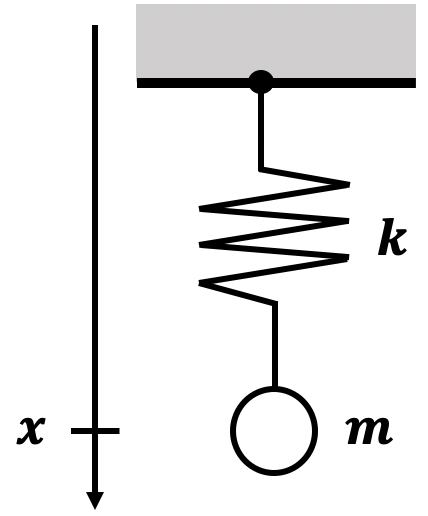
\includegraphics[width=50mm]{fig6_4.png}
\caption[バネ振子によるモデル]{バネ振子によるモデル}
\label{fig6.4}
\end{center}
\end{figure}
この方程式を解くために$z=a{\rm e}^{i\omega t}$とおくと, $\dot{z}=i\omega a{\rm e}^{i\omega t}$, $\ddot{z}=-\omega^2a{\rm e}^{i\omega t}$なので
\begin{equation}
-\omega^2a+2\gamma i\omega a+\omega_0^2a=\omega_0^2a_0.
\end{equation}
これを整理すると
\begin{equation}
a=\frac{\omega_0^2a_0}{\sqrt{(\omega_0^2-\omega^2)^2+4\gamma^2\omega^2}}{\rm e}^{-i\phi}.
\end{equation}
ただし
\begin{equation}
\tan\phi=\frac{2\gamma\omega}{\omega_0^2-\omega^2}.
\end{equation}
これが特解であり, 一般解は外力が0のときの解と合わせたもの\footnote{$\ddot{z}+2\gamma\dot{z}+\omega_0^2z=0$において, 解として$z={\rm e}^{\lambda}t$を仮定して解けばよい. }なので, それは
\begin{equation}
z=a{\rm e}^{-\gamma t}\cos(\omega^{\prime}t+\delta)+\frac{\omega_0^2a_0}{\sqrt{(\omega_0^2-\omega^2)^2+4\gamma^2\omega^2}}\cos(\omega t-\phi).
\label{eq6.8}
\end{equation}
ただし$\omega^{\prime}=\sqrt{\omega_0^2-\gamma^2}$であり, また$a,\delta$は初期条件で決まる値である. \\
\quad 式(\ref{eq6.8})の右辺第1項は十分長い時間で0になるが, 第2項は外力と共に振動を続ける. この振動の振幅
\begin{equation}
|A|=\frac{\omega_0^2a_0}{\sqrt{(\omega_0^2-\omega^2)^2+4\gamma^2\omega^2}},
\end{equation}
を$a_0$で割った値の周波数依存性は図\ref{fig6.5}のようになる. \\
\quad この図より, $\gamma$が非常に小さいときは系が発散し, $\gamma$が小さいとき固有角振動数に近づくと振幅が大きくなるのが分かる(共振). 一方, $\gamma$が大きくなると共振のピークが小さくなっていくが, $\gamma=c/2m$なのでこれは定数$c$を調節することで共振のピークを抑えられる(ダンピングできる)ことを示している. すなわち, ダンピング制御のためには速度に比例した力($c\dot{x}$)を調節するようなフィルタを設計すればよいと分かる. 
\begin{figure}[H]
\begin{center}
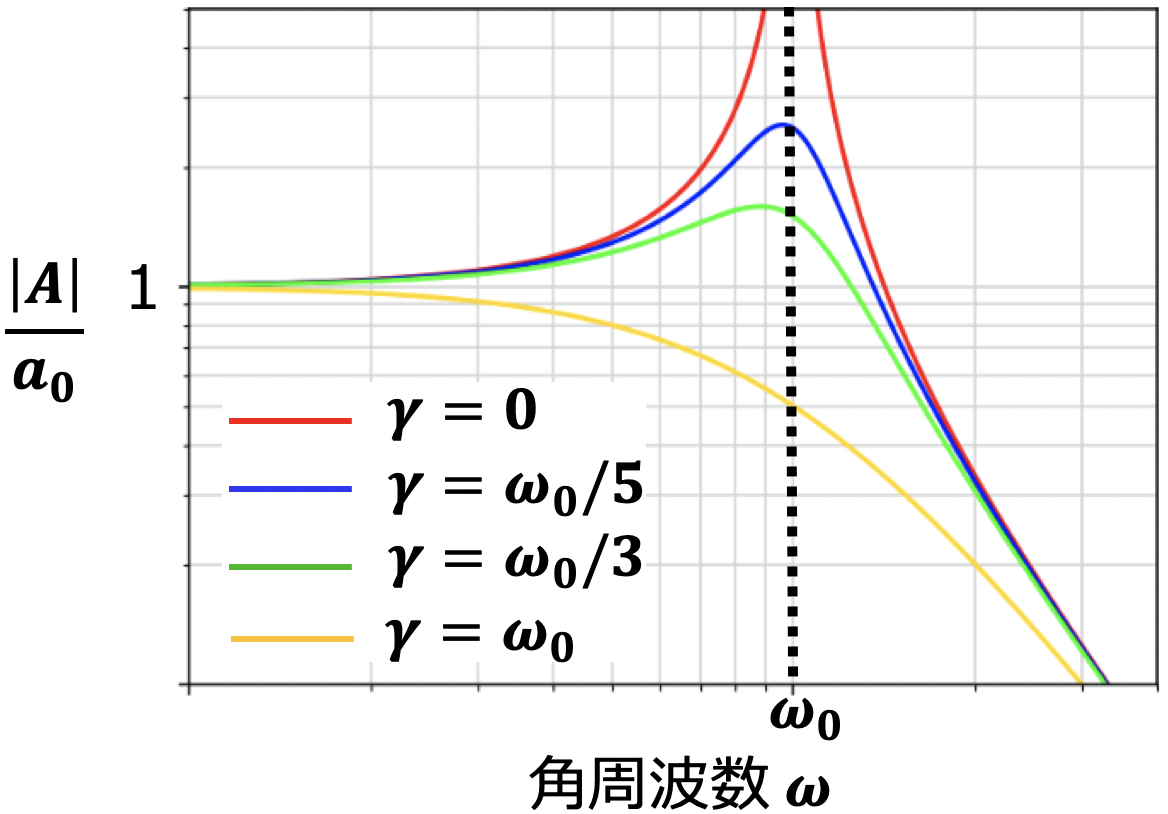
\includegraphics[width=120mm]{fig6_5.png}
\caption[共振の様子を示す曲線]{共振の様子を示す曲線. $\gamma$が大きくなるにつれ, 共振のピークは小さくなっていく. }
\label{fig6.5}
\end{center}
\end{figure}
\begin{figure}[H]
\begin{center}
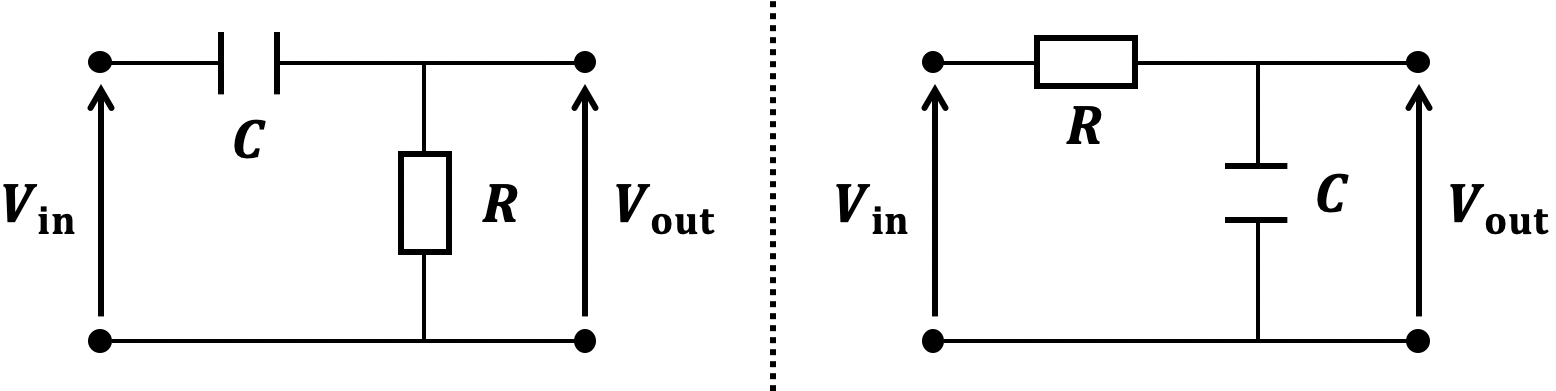
\includegraphics[width=150mm]{fig6_6.png}
\caption[1次のハイパスフィルタ・ローパスフィルタ]{1次のハイパスフィルタ(左)・ローパスフィルタ(右)}
\label{fig6.6}
\end{center}
\end{figure}
ここで, 速度に比例した力を調節するフィルタについて, 典型的な例として1次のハイパスフィルタ・ローパスフィルタを考える. まず1次のハイパスフィルタであるが, コンデンサと抵抗を用いて図\ref{fig6.6}の左側のようになる. 回路に流れる電流を$I$, コンデンサに蓄えられる電荷量をQとすると
\begin{equation}
I=\frac{{\rm d}Q}{{\rm d}t},
\end{equation}
である. 入力信号が入ったとき, コンデンサの両端電圧は$0-V_{\rm in}=-V_{\rm in}$であり, $Q=C\times(-V_{\rm in})$となるので
\begin{equation}
I=\frac{{\rm d}}{{\rm d}t}(-CV_{\rm in})=-C\frac{{\rm d}V_{\rm in}}{{\rm d}t}.
\end{equation}
また, Ohmの法則より$V_{\rm out}=IR$であるから
\begin{equation}
V_{\rm out}=-RC\frac{{\rm d}V_{\rm in}}{{\rm d}t}.
\end{equation}
つまり, ハイパスフィルタを通ると入力信号が微分されて出力される. \\
\quad 例えば入力として大きさ$V_{\rm in}$の矩形波を考えると, 入力の瞬間はコンデンサに電荷が蓄えられないので両端電圧の差は0である. つまり$V_{\rm in}=V_{\rm out}$であり, 抵抗に流れる電流は$I_0=V_{\rm in}/R$となる. この電流によってコンデンサに電荷が蓄えられ, $V_{\rm out}$が徐々に小さくなる. 最終的に矩形波が抜けるとき入力地点の電位が$V_{\rm in}$だけ下がったことになり, これに応じて出力電圧$V_{\rm out}$も$V_{\rm in}$だけ下がる. この後にコンデンサに蓄えられた電荷が放電して入力前の電位に戻る. ここで, 矩形波が時定数$1/RC$に対して十分短ければその形は変わらず出力され, 逆に十分長ければ先に示した通り出力電圧が微分される. つまり, 高周波の信号はそのまま出力するが, 低周波の信号は微分して出力する「ハイパス」フィルタである. \\
\quad 次に1次のローパスフィルタであるが, これもコンデンサと抵抗を用いて図\ref{fig6.6}の右側のように表される. 流れる電流
\begin{equation}
I=\frac{V_{\rm in}}{R},
\end{equation}
によってコンデンサに電荷Qが蓄えられるとすると
\begin{equation}
Q=\int I{\rm d}t,
\end{equation}
であり, このときの出力電圧は
\begin{equation}
V_{\rm out}=-\frac{Q}{C}=-\frac{1}{RC}\int V_{\rm in}{\rm d}t.
\end{equation}
つまり, ローパスフィルタを通ると入力信号が積分されて出力される. \\
\quad 先ほどと同様に大きさ$V_{\rm in}$の矩形波が入力されたとする. その瞬間は出力電圧は0だが, 抵抗$R$を通して電流が流れ徐々に電圧が上がる. その後矩形波が抜ける瞬間はコンデンサの両端の電位差が急に変化するわけではなく, 出力電圧の符号を保ちながら時間と共に放電する. ここで, 矩形波が時定数に対して十分短ければ先に示した通り出力電圧が積分される. 逆に十分長ければその形は変わらず出力される(波形の変化に対してスケールが長い). つまり低周波の信号はそのまま出力するが, 高周波の信号は積分して出力する「ローパス」フィルタである. \\
\quad これらの例をふまえて考えると, 共振ピークのダンピングのためには共振周波数のある領域においてハイパスフィルタがかかるようなフィルタを設計すればよい. すなわちフォトセンサで得た信号を微分してフィードバックすればよいことが分かる. 
\section{ダンピングフィルタの実装とその評価}
\subsection{共振ピークの同定と行列計算}
各懸架装置の各自由度に対し, 共振ピークを同定する必要がある. そのため, まずはアクチュエータで力を加えた際, 懸架系が思い通りの方向に動くかを確認した. これは懸架系の外側にあり, 独立にキャリブレーションされているOpLevの信号を見て行った. その後, アクチュエータで動かした方向とフォトセンサの動作方向の正負が等しいかを確認した後, ホワイトノイズを入れて自由度ごとに励起し, 伝達関数を測定した(図\ref{fig6.7}及び補遺\ref{補遺D}). そこから各自由度の固有モードに対応する共振ピークを特定し, 表\ref{table6.1}$\sim$\ref{table6.4}に示した通りの共振周波数を得た. 
\begin{figure}[H]
\begin{center}
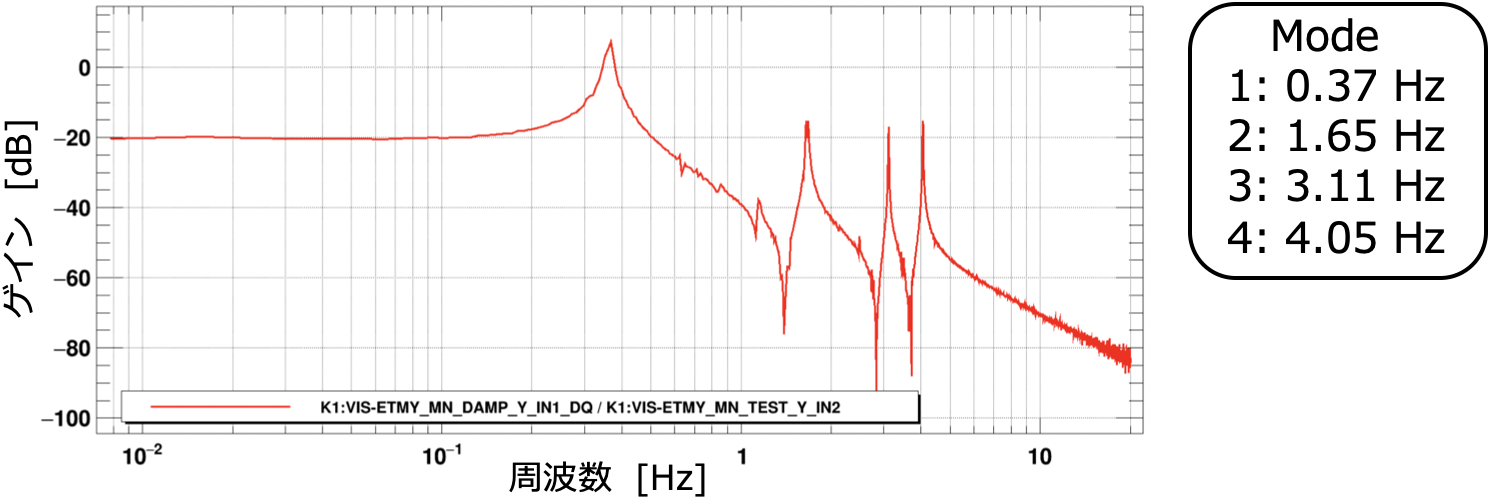
\includegraphics[width=150mm]{fig6_7.png}
\caption[懸架系の応答(ETMY MN Y)]{懸架系の応答(ETMY MN Y). ホワイトノイズを入れてMN段をY方向に励起し, そこからMN段のY方向の動きまでの伝達関数を測定した. 他の懸架系, 自由度の伝達関数については補遺\ref{補遺D}に記した. }
\label{fig6.7}
\end{center}
\end{figure}
\begin{table}[H]
 \centering
  \begin{tabular}{|c||c|c|c|c|}
   \hline
    \diagbox{自由度}{Mode}& 1 & 2 & 3 & 4 \\
   \hline
   L & 0.63 Hz & 1.46 Hz & 2.12 Hz & 2.47 Hz \\
   \hline
   T & 0.63 Hz & 1.49 Hz & 2.12 Hz & 2.49 Hz \\
   \hline
   R & 0.77 Hz & &  &  \\
   \hline
   P & 0.76 Hz & 7.42 Hz &  &   \\
   \hline
   Y & 0.30 Hz & 1.66 Hz & 3.13 Hz & 4.08 Hz \\
   \hline
  \end{tabular}
 \caption[共振周波数 (ETMX)]{共振周波数 (ETMX)}
 \label{table6.1}
\end{table}
\begin{table}[H]
 \centering
  \begin{tabular}{|c||c|c|c|c|}
   \hline
    \diagbox{自由度}{Mode}& 1 & 2 & 3 & 4 \\
   \hline
   L & 0.63 Hz & 1.46 Hz & 2.13 Hz & 2.48 Hz \\
   \hline
   T & 0.63 Hz & 1.52 Hz & 2.09 Hz & 2.516 Hz \\
   \hline
   R & 0.73 Hz & &  &  \\
   \hline
   P & 0.82 Hz & 7.40 Hz &  &   \\
   \hline
   Y & 0.37 Hz & 1.65 Hz & 3.11 Hz & 4.05 Hz \\
   \hline
  \end{tabular}
 \caption[共振周波数 (ETMY)]{共振周波数 (ETMY)}
  \label{table6.2}
\end{table}
\begin{table}[H]
 \centering
  \begin{tabular}{|c||c|c|c|c|}
   \hline
    \diagbox{自由度}{Mode}& 1 & 2 & 3 & 4 \\
   \hline
   L & 0.63 Hz & 1.46 Hz & 2.19 Hz & 2.50 Hz \\
   \hline
   T & 0.63 Hz & 1.45 Hz & 2.13 Hz & 2.49 Hz \\
   \hline
   R & 0.76 Hz & &  &  \\
   \hline
   P & 0.85 Hz & 7.39 Hz &  &   \\
   \hline
   Y & 0.30 Hz & 1.67 Hz & 3.09 Hz & 4.09 Hz \\
   \hline
  \end{tabular}
 \caption[共振周波数 (ITMX)]{共振周波数 (ITMX)}
  \label{table6.3}
\end{table}
\begin{table}[H]
 \centering
  \begin{tabular}{|c||c|c|c|c|}
   \hline
    \diagbox{自由度}{Mode}& 1 & 2 & 3 & 4 \\
   \hline
   L & 0.6328 Hz & 1.461 Hz & 2.188 Hz & 2.500 Hz \\
   \hline
   T & 0.6250 Hz & 1.469 Hz & 2.156 Hz & 2.500 Hz \\
   \hline
   R & 0.7500 Hz & &  &  \\
   \hline
   P & 0.8516 Hz & 7.391 Hz &  &   \\
   \hline
   Y & 0.2969 Hz & 1.672 Hz & 3.094 Hz & 4.086 Hz \\
   \hline
  \end{tabular}
 \caption[共振周波数 (ITMY)]{共振周波数 (ITMY)}
  \label{table6.4}
\end{table}
また, ダンピングフィルタは各自由度に対してかけるので, 自由度ごとに対応するようにフォトセンサの信号を合成している. ここで, フォトセンサが懸架装置の揺れを正確に検知して同程度の出力をすれば, 信号の合成はセンサの幾何学的な配置で決まる. また, アクチュエータについても同様に, 入出力の関係が同じ場合は幾何学的配置に基づいて信号の合成を行えば, それぞれの自由度に対して個別に力を加えることができる. \\
\quad しかし, 自由度にはカップリングが存在し, ある自由度にのみ力を加えるつもりでも, 他の自由度が動いてしまうということがある. よって, 対象の自由度以外に対してダンピング制御を行わないよう, 自由度ごとのカップリングを以下のようにして求める必要がある. \\
\quad まず, 懸架装置を共振周波数で揺らし続ける. この際, その周波数に共振ピークを持たない自由度の揺れは励起されないが, 共振ピークを持つ場合は徐々に揺れが大きくなる. それらの自由度に対し, 揺れの大きさの比を取り, それを打ち消す(decouplingする)ように式(\ref{eq6.16})に示す行列の非対角成分を求める. 
\begin{equation}
\begin{pmatrix}
L^{\prime} \\
T^{\prime} \\
V^{\prime} \\ 
R^{\prime} \\
P^{\prime}\\
Y^{\prime}
\end{pmatrix}=
\begin{pmatrix}
1&C_{TL}&C_{VL}&C_{RL}&C_{PL}&C_{YL}\\
C_{LT}&1&C_{VT}&C_{RT}&C_{PT}&C_{YT}\\
C_{LV}&C_{TV}&1&C_{RV}&C_{PV}&C_{YV}\\
C_{LR}&C_{TR}&C_{VR}&1&C_{PR}&C_{YR}\\
C_{LP}&C_{TP}&C_{VP}&C_{RP}&1&C_{YP} \\
C_{LY}&C_{TY}&C_{VY}&C_{RY}&C_{PY}&1
\end{pmatrix}
\begin{pmatrix}
L\\
T\\
V \\ 
R \\
P \\
Y
\end{pmatrix}.
\label{eq6.16}
\end{equation}
ただし, プライム付き文字が上記の測定で得られた自由度, そうでない文字が真の自由度であり, 非対角成分が自由度ごとのカップリングを表している. 
\subsection{ダンピングフィルタの実装とその効果}
\ref{sec6.2}節で示した通り, 共振周波数が存在する周波数領域において信号を微分して系に返すフィルタを作成すればダンピング制御を実現できる. そこで, フォトセンサで得られた信号に対してそのような動作を行うフィルタをインストールした. 図\ref{fig6.8}はETMXのL方向に対するフィルタを示したものである. \\
\quad 10 Hzあたりまでは共振周波数での振動を抑えるためにハイパスフィルタをかけている. 具体的には25 Hzに極を, 0 Hzに零点を設定しており, この部分が鏡の速度に比例した力を系にフィードバックしている. \\
\quad 一方, ダンピング制御が必要ないそれ以降の周波数領域ではノイズを減らすため\footnote{フィードバック制御におけるノイズについては第\ref{第7章}章参照. }にローパスフィルタをかけている. \\
\quad また, 図\ref{fig6.9}は前小節で記したダンピングフィルタをかけた上で, 励起信号からMNの動きまでの伝達関数を測定した結果を示している. 赤線はフィルタなしの場合であるが, この時は共振周波数において, 揺れが大きくなっているのが分かる. しかし, ダンピングフィルタをかけると青線で示された通り, その揺れが抑えられている. これより, 地震などの何らかの理由により低温懸架装置の共振が励起された場合でも, このフィルタがかけられていれば, その共振をダンプすることができると言える. 
\begin{figure}[H]
\begin{center}
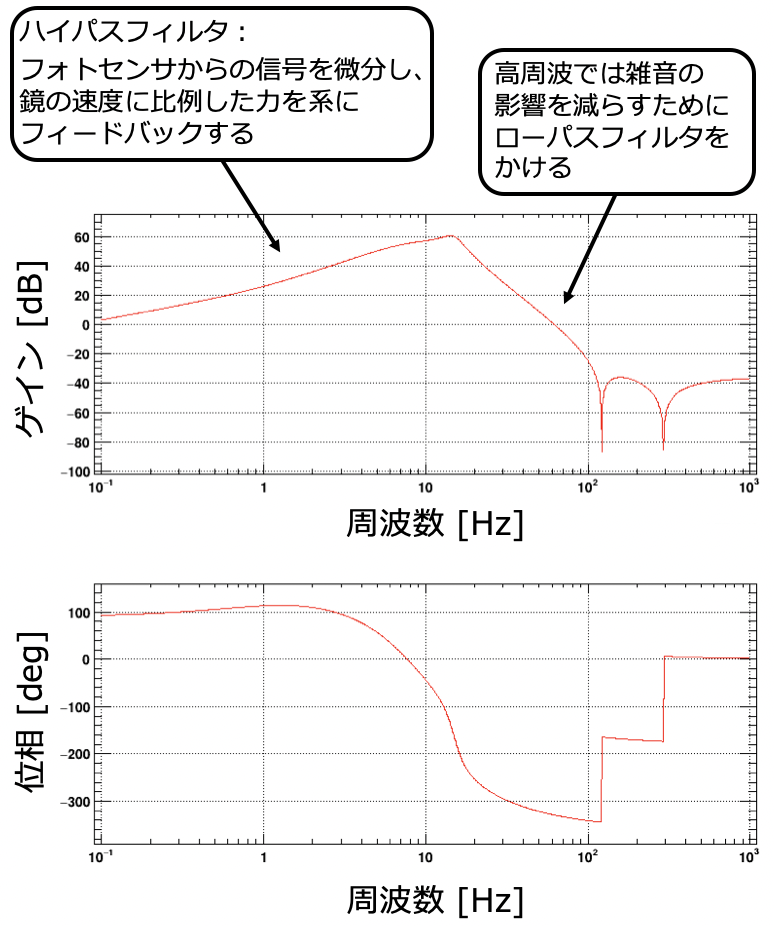
\includegraphics[width=100mm]{fig6_8.png}
\caption[ダンピングフィルタ]{ダンピングフィルタの例(ETMY MN Y). ダンピングしたい共振周波数が存在する低周波では, 鏡の速度に比例した力を系にフィードバックするためのハイパスフィルタをかけている. 一方, 高周波ではノイズの影響を抑えるためにローパスフィルタをかけた. }
\label{fig6.8}
\end{center}
\end{figure}
\begin{figure}[H]
\begin{center}
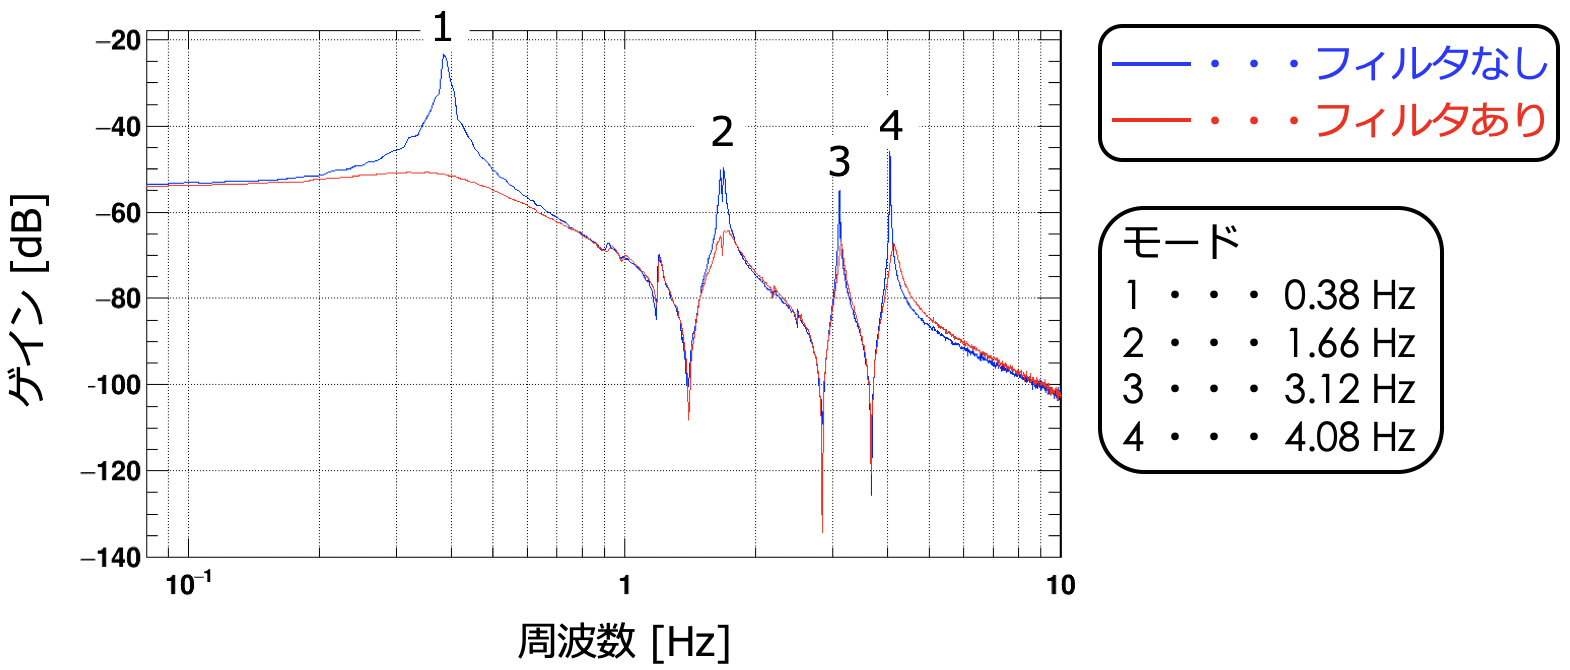
\includegraphics[width=150mm]{fig6_9.png}
\caption[ダンピングフィルタをかけた時の伝達関数]{ダンピングフィルタをかけた時の伝達関数(ETMY MN段についてY方向に励起し, そこからMN段のY方向の動きまでの伝達関数を測定した). フィルタをかけた場合(青)はフィルタなしの場合(赤)に比べて共振周波数における揺れが抑制されているのが分かる. }
\label{fig6.9}
\end{center}
\end{figure}
\subsection{1/e減衰時間によるダンピング制御の評価}
共振周波数における揺れを抑えられることは分かったが, その抑制にどれだけ時間を要するかという点も, 観測状態への素早い復帰という点で重要である. これは図\ref{fig3.6}に示したCalm-down Phaseにおいて, 各共振モードの振幅が1/eに減衰する時間によって評価される. ここでは5.2.3.1で示したように, 共振周波数に等しい周波数の励起信号を入れた後でその励起を止め, 振動が減衰する時間を測る, という方法で測定を行った. \\
\quad 図\ref{fig6.10}はETMYのYのモード4 (4.08 Hz) の共振について, 励起した揺れが収まるまでの時間をダンピング制御なし, ありの場合で比較したものである. 青線はダンピング制御なしの場合であり, 励起した揺れの振幅が1/eに収まるまでに約97 秒かかっていることが分かった. 一方, ダンピング制御をかけた際の減衰の様子は赤線で示された通りで, 約2 秒で振幅が1/eに収まっているのが分かる. Calm-down Phaseにおける減衰時間に対する要求値は60 秒とされているので, これは十分早く振動を抑えられていると言える. 
\begin{figure}[H]
\begin{center}
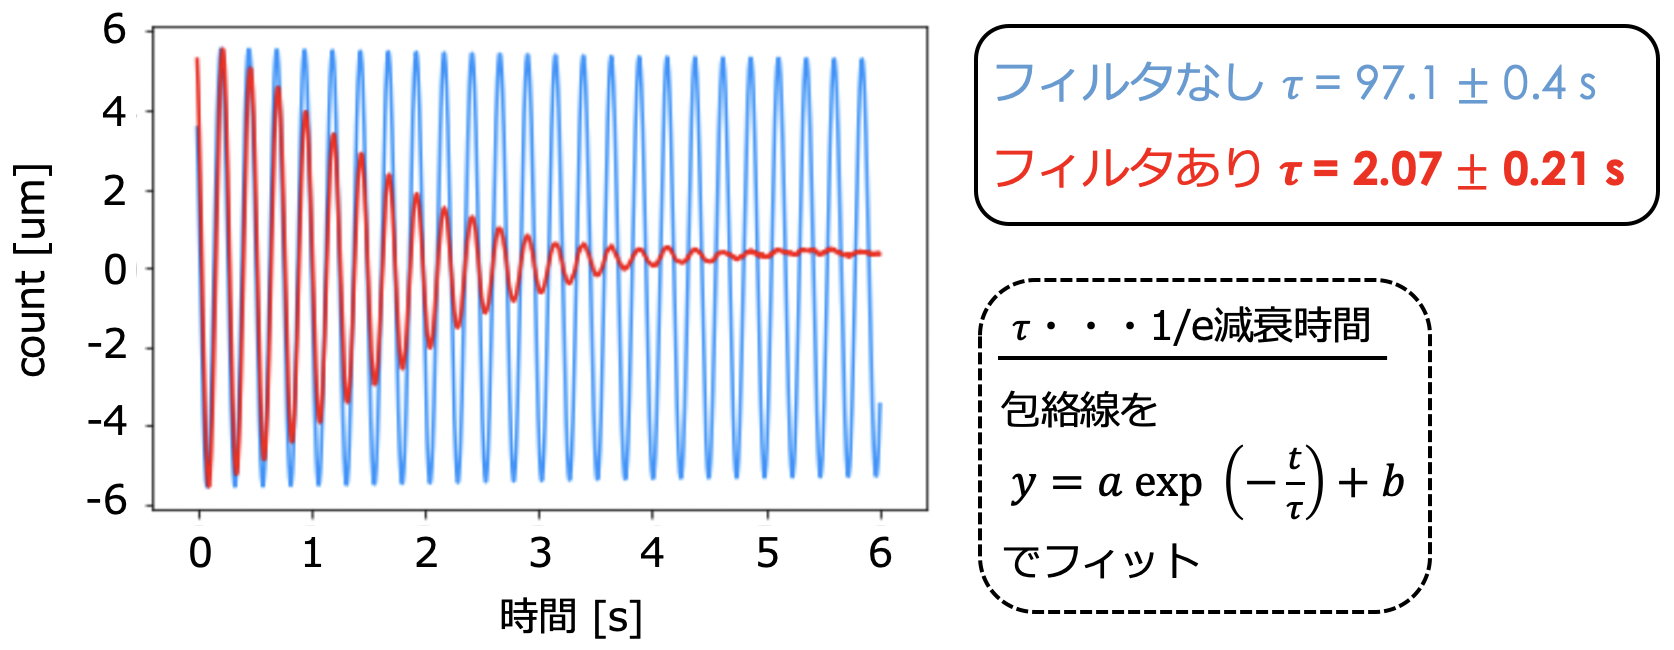
\includegraphics[width=150mm]{fig6_10.png}
\caption[励起した共振が収まる様子]{励起した共振が収まる様子. ダンピング制御なし(青)の場合は振動が収まるまでに約97 秒待つ必要があるが, 制御をかけた場合(赤)はそれが2 秒程度に短縮される. }
\label{fig6.10}
\end{center}
\end{figure}
\quad 同様の測定を懸架装置, 自由度に対しても行った(全て常温). 図\ref{fig6.11}$\sim$\ref{fig6.14}および表\ref{table6.5}$\sim$\ref{table6.8}はその結果をまとめたもので, ダンピング制御なしの場合(青点)およびダンピング制御ありの場合(赤点)の, 1/e減衰時間の変化を示している. また, 図中の緑線はCalm-down Phaseにおける減衰時間に対する要求値(60秒)である. \\
\quad これより, 各懸架装置の各自由度の各モードに対して, 要求値を十分満たすダンピング制御を行うことができていると言える. これは外乱などで干渉計のロックが失われた場合でも速やかに再ロックすることが可能であることを意味し, 観測時間の増加につながると期待される. 
\begin{figure}[H]
\begin{center}
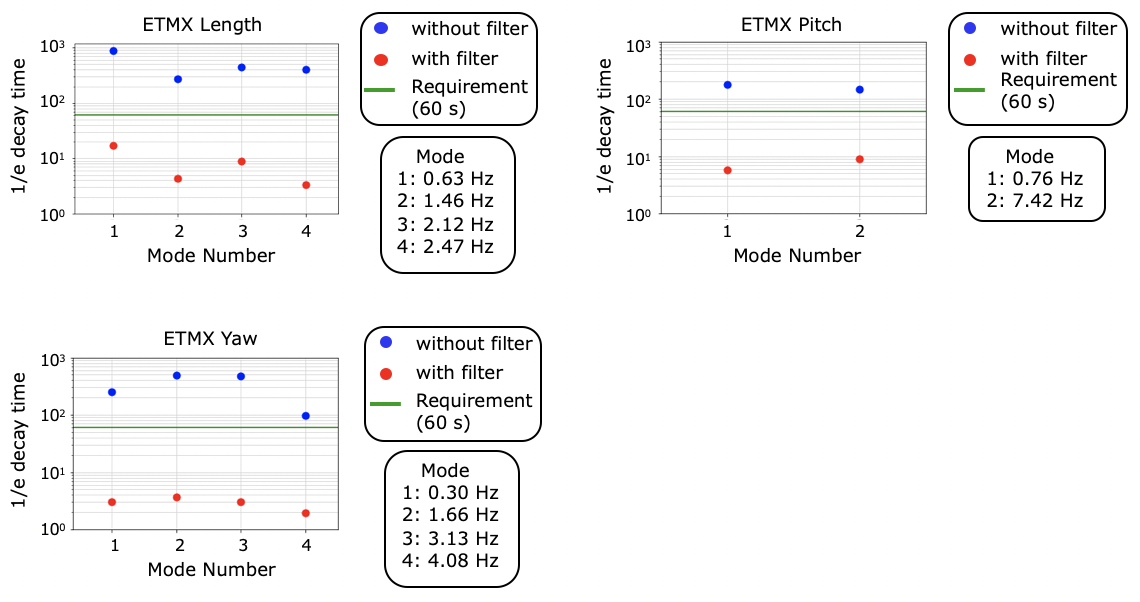
\includegraphics[width=175mm]{fig6_11.png}
\caption[1/e減衰時間 (ETMX)]{ダンピングフィルタあり / なしの1/e減衰時間の比較 (ETMX). 青色, 赤色の点がそれぞれダンピングフィルタなし, ありの時の結果を示している. なお, 緑線はLock-acquisition phaseにおける要求値を示しており, ダンピングフィルタを用いると十分早く外乱が抑制されることがこの図から分かる. }
\label{fig6.11}
\end{center}
\end{figure}
\begin{figure}[H]
\begin{center}
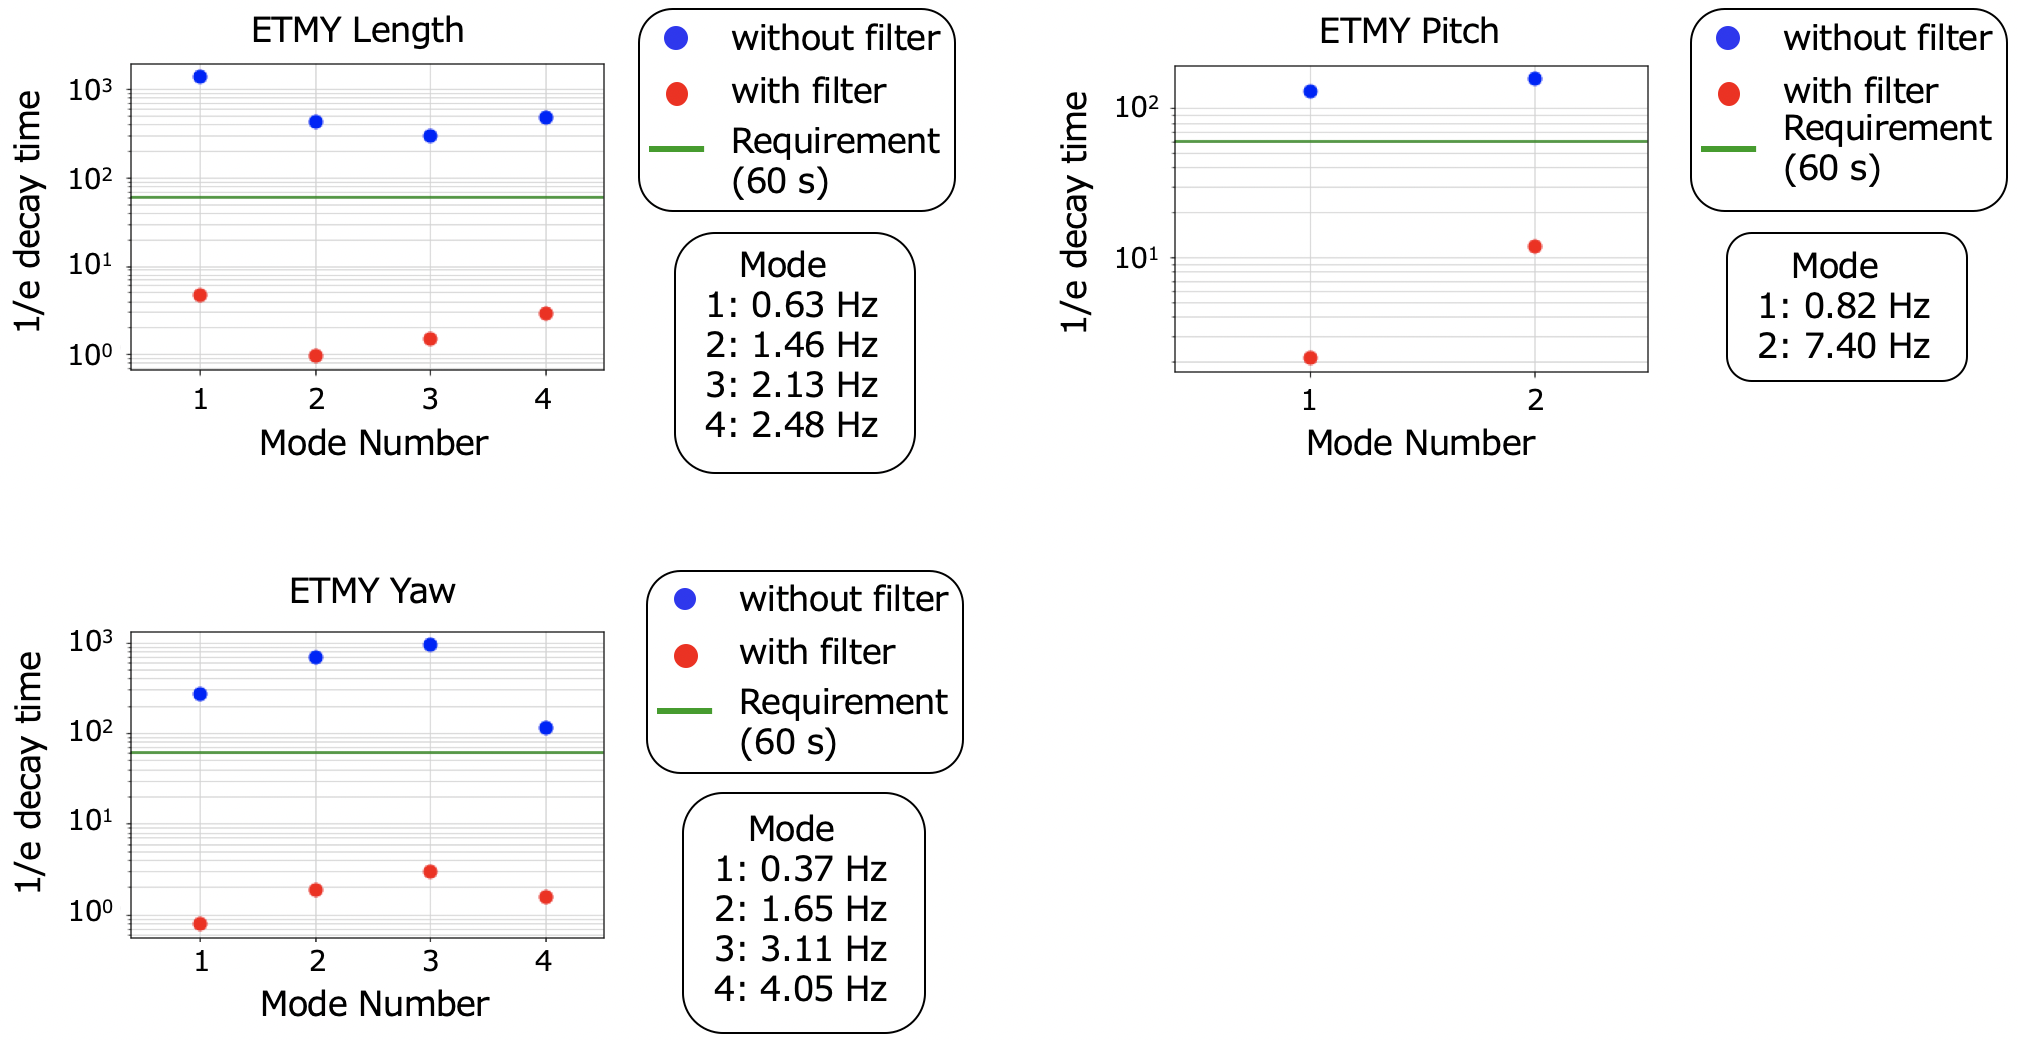
\includegraphics[width=175mm]{fig6_12.png}
\caption[1/e減衰時間 (ETMY)]{ダンピングフィルタあり / なしの1/e減衰時間の比較 (ETMY). 青色, 赤色の点がそれぞれダンピングフィルタなし, ありの時の結果を示している. なお, 緑線はLock-acquisition phaseにおける要求値を示しており, ダンピングフィルタを用いると十分早く外乱が抑制されることがこの図から分かる. }
\label{fig6.12}
\end{center}
\end{figure}
\begin{figure}[H]
\begin{center}
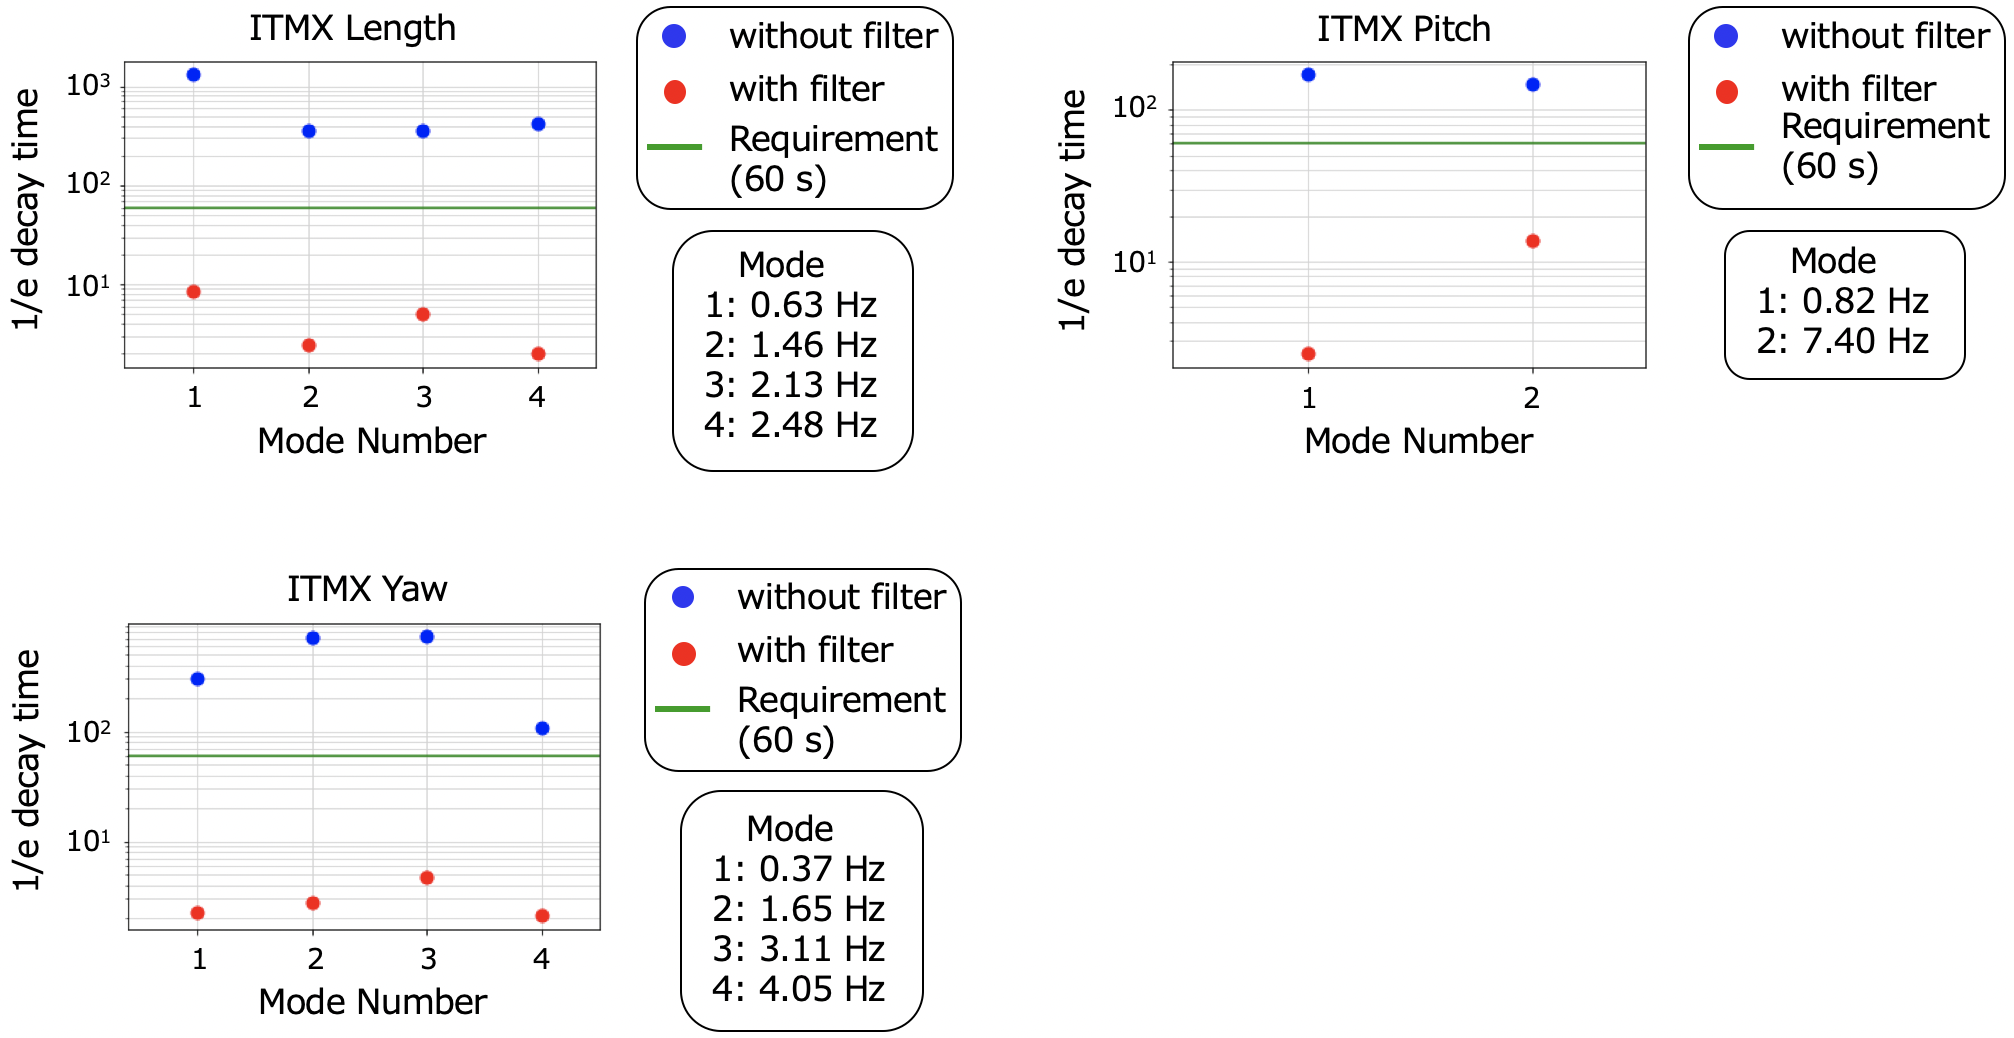
\includegraphics[width=175mm]{fig6_13.png}
\caption[1/e減衰時間 (ITMX)]{ダンピングフィルタあり / なしの1/e減衰時間の比較 (ITMX). 青色, 赤色の点がそれぞれダンピングフィルタなし, ありの時の結果を示している. なお, 緑線はLock-acquisition phaseにおける要求値を示しており, ダンピングフィルタを用いると十分早く外乱が抑制されることがこの図から分かる. }
\label{fig6.13}
\end{center}
\end{figure}
\begin{figure}[H]
\begin{center}
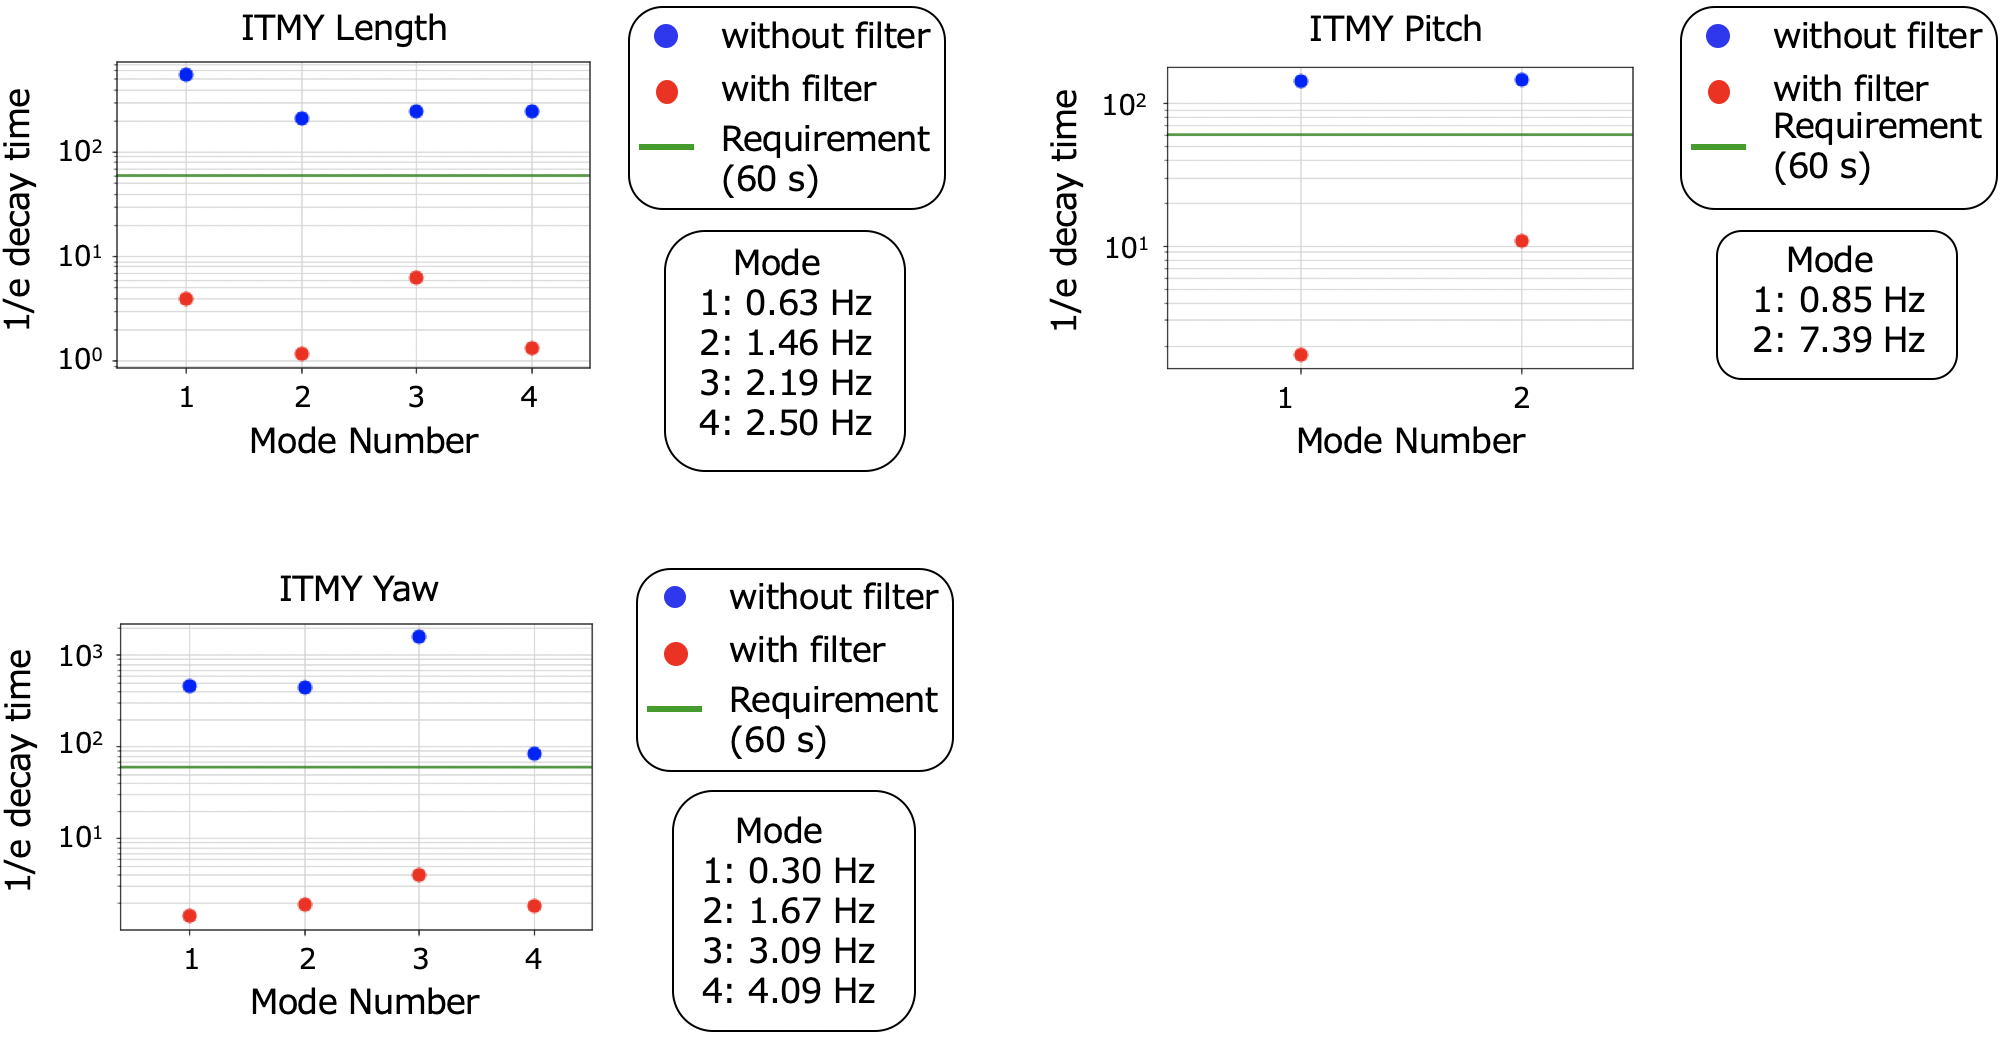
\includegraphics[width=175mm]{fig6_14.png}
\caption[1/e減衰時間 (ITMY)]{ダンピングフィルタあり / なしの1/e減衰時間の比較 (ITMY). 青色, 赤色の点がそれぞれダンピングフィルタなし, ありの時の結果を示している. なお, 緑線はLock-acquisition phaseにおける要求値を示しており, ダンピングフィルタを用いると十分早く外乱が抑制されることがこの図から分かる. }
\label{fig6.14}
\end{center}
\end{figure}
\begin{table}[H]
 \centering
  \begin{tabular}{|c||c|c|c|c|c|}
   \hline
    & フィルタ & Mode 1 & Mode 2 & Mode 3 & Mode 4 \\
   \hline
   \multirow{2}{*}{L} & なし &(8.921 $\pm$ 0.174)$\times10^2$ s & (2.702 $\pm$ 0.004)$\times10^2$ s & (4.474 $\pm$ 0.046)$\times10^2$ s & (4.057 $\pm$ 0.007)$\times10^2$ s \\
   \cline{2-6}
      & あり &(1.740 $\pm$ 0.076)$\times10^1$ s & 4.382 $\pm$ 0.706 s & 4.620 $\pm$ 0.296 s & 3.315 $\pm$ 0.555  s \\
   \hline\hline
   \multirow{2}{*}{P} & なし &(1.788 $\pm$ 0.028)$\times10^2$ s & (1.485 $\pm$ 0.001)$\times10^2$ s &  & \\
   \cline{2-6}
      & あり & 5.708 $\pm$ 0.263 s & 8.975 $\pm$ 0.150 s & & \\
   \hline\hline
   \multirow{2}{*}{Y} & なし &(2.509 $\pm$ 0.003)$\times10^2$ s & (4.978 $\pm$ 0.062)$\times10^2$ s & (4.793 $\pm$ 0.023)$\times10^2$ s & (9.708 $\pm$ 0.015)$\times10^1$ s \\
   \cline{2-6}
      & あり & 3.012 $\pm$ 0.227 s & 3.623 $\pm$ 0.086 s & 3.038 $\pm$ 0.105 s & 1.968 $\pm$ 0.212 s \\
   \hline
  \end{tabular}
 \caption[1/e 減衰時間 (ETMX)]{1/e 減衰時間 (ETMX)}
 \label{table6.5}
\end{table}
\begin{table}[H]
 \centering
  \begin{tabular}{|c||c|c|c|c|c|}
   \hline
    & フィルタ & Mode 1 & Mode 2 & Mode 3 & Mode 4 \\
   \hline
   \multirow{2}{*}{L} & なし &(1.381 $\pm$ 0.003)$\times10^3$ s & (4.310 $\pm$ 0.006)$\times10^2$ s & (3.047 $\pm$ 0.028)$\times10^2$ s & (4.790 $\pm$ 0.002)$\times10^2$ s \\
   \cline{2-6}
      & あり &4.691 $\pm$ 0.090 s & (9.685 $\pm$ 0.833)$\times10^{-1}$ s & 1.490 $\pm$ 0.281 s & 2.959 $\pm$ 0.572 s \\
   \hline\hline
   \multirow{2}{*}{P} & なし &(1.313 $\pm$ 0.001)$\times10^2$ s & (1.572 $\pm$ 0.001)$\times10^2$ s & &\\
   \cline{2-6}
     & あり &2.141 $\pm$ 0.027 s & (1.201 $\pm$ 0.007)$\times10^{1}$ s & & \\
   \hline\hline
   \multirow{2}{*}{Y} & なし &(2.691 $\pm$ 0.024)$\times10^2$ s & (6.872 $\pm$ 0.169)$\times10^2$ s & (9.353 $\pm$ 0.025)$\times10^2$ s & (1.167 $\pm$ 0.006)$\times10^2$ s \\
   \cline{2-6}
      & あり &(7.999 $\pm$ 0.024)$\times10^{-1}$ s & 1.921 $\pm$ 0.239 s & 3.057 $\pm$ 0.164 s & 1.560 $\pm$ 0.121 s \\
   \hline
  \end{tabular}
   \caption[1/e 減衰時間 (ETMY)]{1/e 減衰時間 (ETMY)}
    \label{table6.6}
\end{table}
\begin{table}[H]
 \centering
  \begin{tabular}{|c||c|c|c|c|c|}
   \hline
    & フィルタ & Mode 1 & Mode 2 & Mode 3 & Mode 4 \\
   \hline
   \multirow{2}{*}{L} & なし &(1.305 $\pm$ 0.022)$\times10^3$ s & (3.523 $\pm$ 0.014)$\times10^2$ s & (3.585 $\pm$ 0.096)$\times10^2$ s & (4.276 $\pm$ 0.096)$\times10^2$ s \\
   \cline{2-6}
      & あり &8.692 $\pm$ 0.695 s & 2.429 $\pm$ 0.714 s & 5.088 $\pm$ 0.135 s & 2.020 $\pm$ 0.454 s \\
   \hline\hline
   \multirow{2}{*}{P} & なし &(1.710 $\pm$ 0.109)$\times10^2$ s & (1.493 $\pm$ 0.001)$\times10^2$ s & &  \\
   \cline{2-6}
     & あり & 2.475 $\pm$ 0.123 s & (1.369$\pm$0.004)$\times10^1$ s & &  \\
   \hline\hline
   \multirow{2}{*}{Y} & なし &(3.026 $\pm$ 0.037)$\times10^2$ s & (7.105 $\pm$ 0.043)$\times10^2$ s & (7.260 $\pm$ 0.202)$\times10^2$ s & (1.067 $\pm$ 0.006)$\times10^2$ s \\
   \cline{2-6}
      & あり &2.228 $\pm$ 0.075 s & 2.788 $\pm$ 0.161 s & 4.659 $\pm$ 0.085 s & 2.118 $\pm$ 0.084 s \\
   \hline
  \end{tabular}
  \caption[1/e 減衰時間 (ITMX)]{1/e 減衰時間 (ITMX)}
   \label{table6.7}
\end{table}
\begin{table}[H]
 \centering
    \begin{tabular}{|c||c|c|c|c|c|}
   \hline
    & フィルタ & Mode 1 & Mode 2 & Mode 3 & Mode 4 \\
   \hline
   \multirow{2}{*}{L} & なし &(5.475 $\pm$ 0.065)$\times10^2$ s & (2.126 $\pm$ 0.004)$\times10^2$ s & (2.435 $\pm$ 0.027)$\times10^2$ s & (2.446 $\pm$ 0.070)$\times10^2$ s \\
   \cline{2-6}
      & あり &3.890 $\pm$ 0.110 s & 1.169 $\pm$ 0.150 s & 6.251 $\pm$ 0.152 s & 1.318 $\pm$ 0.256 s \\
   \hline\hline
   \multirow{2}{*}{P} & なし &(1.455 $\pm$ 0.035)$\times10^2$ s & (1.457 $\pm$ 0.001)$\times10^2$ s & &   \\
   \cline{2-6}
     & あり &1.724 $\pm$ 0.114 s & (1.093 $\pm$ 0.006)$\times10^{1}$ s & &  \\
   \hline\hline
   \multirow{2}{*}{Y} & なし &(4.674 $\pm$ 0.005)$\times10^2$ s & (4.553 $\pm$ 0.117)$\times10^2$ s & (1.587 $\pm$ 0.008)$\times10^3$ s & (8.667 $\pm$ 0.001)$\times10^2$ s \\
   \cline{2-6}
      & あり &1.441 $\pm$ 0.011 s & 1.942 $\pm$ 0.074 s & 3.994 $\pm$ 0.177 s & 1.859 $\pm$ 0.071 s \\
   \hline
  \end{tabular}
  \caption[1/e 減衰時間 (ITMY)]{1/e 減衰時間 (ITMY)}
   \label{table6.8}
\end{table}
\section{冷却した際の制御の変更}
第\ref{第5章}章において測定した82 KにおけるETMXの伝達関数, 共振周波数を測定した. 伝達関数の形に大きな変化は見られず, また共振周波数は数パーセント高くなっただけであり, それによるUGFでの位相余裕の変化は少なかった. そこで, 297 Kでのダンピング制御のゲインだけを変えて82 Kにおける1/e 減衰時間を測定したところ図\ref{fig6.15}および表\ref{table6.9}のようになった. 
\begin{figure}[H]
\begin{center}
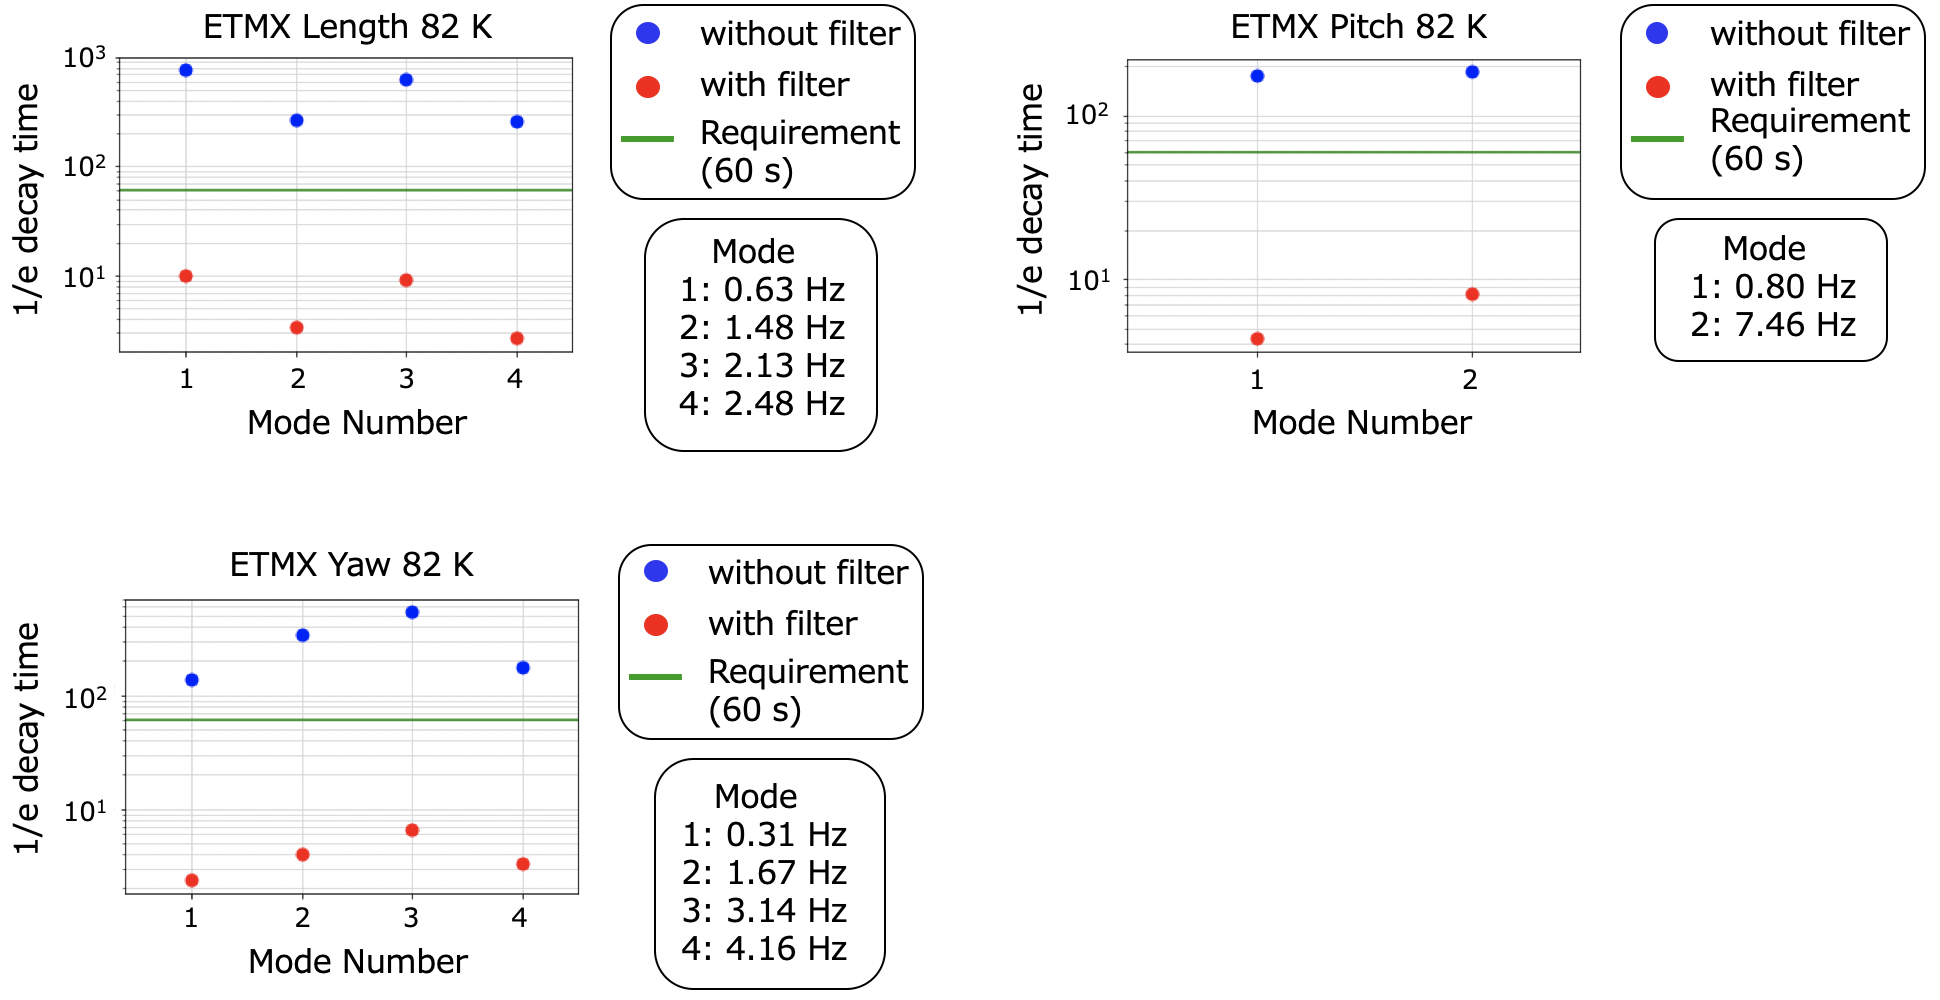
\includegraphics[width=175mm]{fig6_15.png}
\caption[82 Kにおける1/e減衰時間 (ETMX)]{82 Kにおけるダンピングフィルタあり / なしの1/e減衰時間の比較 (ETMX). 青色, 赤色の点がそれぞれダンピングフィルタなし, ありの時の結果を示している. 297 Kの場合の制御からゲインを変更しただけであるが, 要求に対して十分早く振動を抑えることができており, 冷却によってダンピング制御に大幅な変更を加える必要がないことが分かる. }
\label{fig6.15}
\end{center}
\end{figure}
\begin{table}[H]
 \centering
  \begin{tabular}{|c||c|c|c|c|c|}
   \hline
    & フィルタ & Mode 1 & Mode 2 & Mode 3 & Mode 4 \\
   \hline
   \multirow{2}{*}{L} & なし &(7.569 $\pm$ 0.070)$\times10^2$ s & (2.629 $\pm$ 0.008)$\times10^2$ s & (6.312 $\pm$ 0.009)$\times10^2$ s & (2.555 $\pm$ 0.004)$\times10^2$ s \\
   \cline{2-6}
      & あり &(1.014$\pm$0.097)$\times10^1$ s & 3.366 $\pm$ 0.932 s & 9.279 $\pm$ 0.433 s & 2.683 $\pm$ 0.578 s \\
   \hline\hline
   \multirow{2}{*}{P} & なし &(1.745 $\pm$ 0.004)$\times10^2$ s & (1.839 $\pm$ 0.002)$\times10^2$ s & &  \\
   \cline{2-6}
     & あり & 4.342 $\pm$ 0.017 s & 8.057 $\pm$ 0.129 s & &  \\
   \hline\hline
   \multirow{2}{*}{Y} & なし &(1.377 $\pm$ 0.007)$\times10^2$ s & (3.414 $\pm$ 0.003)$\times10^2$ s & (5.373 $\pm$ 0.002)$\times10^2$ s & (1.754 $\pm$ 0.001)$\times10^2$ s \\
   \cline{2-6}
      & あり &2.377 $\pm$ 0.245 s & 3.980 $\pm$ 0.232 s & 6.555 $\pm$ 0.156 s & 3.327 $\pm$ 0.063 s \\
   \hline
  \end{tabular}
  \caption[1/e 減衰時間 (ETMX 82 K)]{1/e 減衰時間 (ETMX 82 K)}
   \label{table6.9}
\end{table}
これより, 297 Kにおけるダンピング制御のゲインを変えるだけで, 82 Kでも60 秒以内に振動がおさまるという要求を十分満たすことができると言える. つまり, 冷却に伴う懸架装置の特性の変化により, 制御の大幅な変更の必要性は生じず, ゲインを調整するだけで良いことが分かった.